Линейная автономная система второго порядка записывается так:
\begin{equation}\label{autonom-sys-2d}
    \begin{cases}
    \dot{x_1} = a_{11} x_1 + a_{12} x_2 \\
    \dot{x_2} = a_{21} x_1 + a_{22} x_2
    \end{cases}
\end{equation}

Также удобно обозначить \(x = x_1, y = x_2\). Числа \(a_{11}, a_{12}, a_{21}, a_{22}\)~--- заданные действительные числа, \(t \in R_t^1\). Введем матрицу 
\[A = \begin{pmatrix} a_{11} & a_{12} \\ a_{21} & a_{22}\end{pmatrix}.\]

\begin{definition}
Линейная автономная система~(\ref{autonom-sys-2d}) называется простой, если матрица $A$ — невырожденна. В противном случае система~(\ref{autonom-sys-2d}) называется сложной.
\end{definition}

\begin{lemmanote}
Если задано автономное уравнение второго порядка
\begin{equation}
    \ddot{x} + a \dot{x} + b x = 0
\end{equation}
с действительными коэфициентами $a, b$, то его положениями равновесия называются положения равновесия автономной системы вида
\begin{equation}
\begin{cases}
\dot{x} = y\\
\dot{y} = -bx - ay.
\end{cases}
\end{equation}
\end{lemmanote}

Рассмотрим различные случаи. Далее, $\lambda_1, \lambda_2$~--- собственные значения матрицы $A$, a $h_1, h_2$~--- соответсвтующие собственные векторы. 

\paragraph{Случай простой системы}

\begin{enumerate}
    \item Случай действительных $\lambda_1, \lambda_2$.\\
        Если они различны, то существует базис из собственных векторов. Все действительные решения задаются формулой
        \[x(t) = c_1 e^{\lambda_1 t} h_1 + c_2 e^{\lambda_2 t} h_2.\] В базисе из собственных векторов координаты решения \(x(t)\) системы~(\ref{autonom-sys-2d}) имеют вид
        \[\zeta_1 = c_1 e^{\lambda_1 t},\;\; \zeta_2 =  c_2 e^{\lambda_2 t}.\] В силу симметрии, достаточно исследовать систему при $\zeta_1 > 0, \zeta_2 > 0.$
        \begin{enumerate}
        \item Пусть $\lambda_1$ < 0, $\lambda_2$ < 0 и $|\lambda_1| < |\lambda_2|$.\\
        Тогда:
        \begin{itemize}
        \item $c_1 = c_2 = 0$ дает положение равновесия $x = 0$;
        \item $c_1 >0, c_2 = 0$ дает полуось $\zeta_1 > 0$, причем $\zeta_1 \longrightarrow +0, t \longrightarrow +\infty$;
        \item $c_1 = 0, c_2 > 0$ дает полуось $\zeta_2 > 0$, причем $\zeta_2 \longrightarrow +0, t \longrightarrow +\infty$;
        \item $c_1 > 0, c_2 > 0$, то 
        \[e^t = \Big(\frac{\zeta_1}{c_1}\Big)^{\frac{1}{\lambda_1}} \;\; \Rightarrow \;\; \zeta_2 = c \zeta_1^{\alpha}, \quad c = c_2 \cdot c_1^{-\frac{\lambda_2}{\lambda_1}}, \quad \alpha = \frac{\lambda_2}{\lambda_1} > 1.\]
        В этом случае траектории являются кривыми типа ветвей параболы, касающихся в пределе при $t \longrightarrow +\infty$ оси $\zeta_1$ в начале координат.
        \end{itemize}
        В целом в случае (a) получаем семейство фазовых траекторий типа ветвей параболы и пять специальных траекторий: положение равновесия $x = 0$ и четыре полуоси осей координат $\zeta_1, \zeta_2$. Схематически фазовый портрет системы~(\ref{autonom-sys-2d}) в случае (a) показан на рисунке ниже.\\
        Стрелка на траектории показывает направление движения при $t \longrightarrow +\infty$.
        В этом случае положение равновесия $x = 0$ называется \textbf{устойчивым узлом} системы~(\ref{autonom-sys-2d}).
        
    \item Пусть $\lambda_1$ > 0, $\lambda_2$ > 0 и $|\lambda_1| < |\lambda_2|$.\\
        Меняется лишь направление движения по траекториям. В данном случае положение равновесия называется \textbf{неустойчивым узлом}. Схематически фазовый портрет системы~(\ref{autonom-sys-2d}) в случае (b) показан на рисунке ниже.
        \begin{figure}[H]\label{autonom-casea}
            \centering
            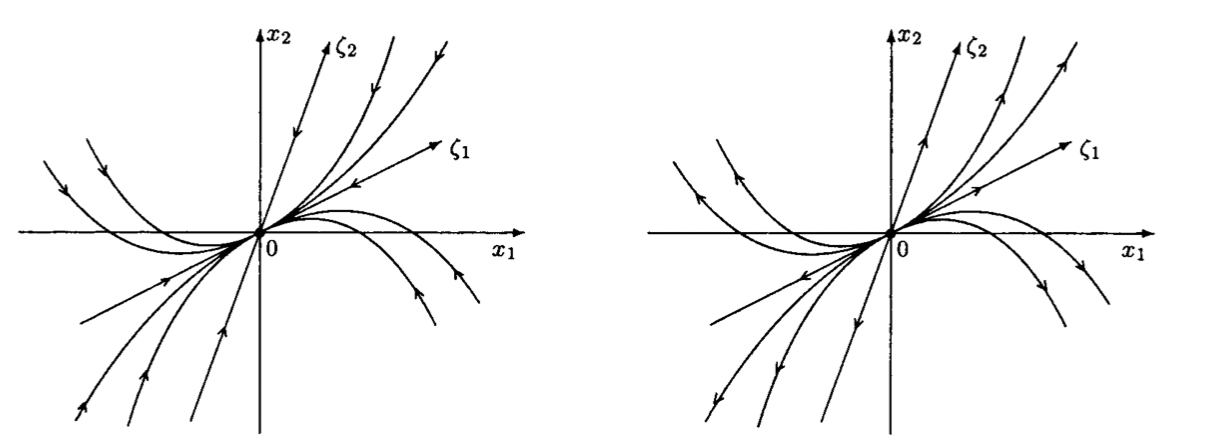
\includegraphics[scale=0.8]{sections/Sasha/images/autonom-casea.png}
            \caption{Слева $\lambda_1$ < 0, $\lambda_2$ < 0 и $|\lambda_1| < |\lambda_2|$, справа $\lambda_1$ > 0, $\lambda_2$ > 0 и $|\lambda_1| < |\lambda_2|$}
        \end{figure}
        
    \item Пусть \(\lambda_1 < 0 < \lambda_2\).\\
        Тогда 
        \begin{itemize}
        \item $c_1 = c_2 = 0$ дает положение равновесия $x = 0$;
        \item $c_1 >0, c_2 = 0$ дает полуось $\zeta_1 > 0$, причем $\zeta_1 \longrightarrow +0, t \longrightarrow +\infty$;
        \item $c_1 = 0, c_2 > 0$ дает полуось $\zeta_2 > 0$, причем $\zeta_2 \longrightarrow +\infty, t \longrightarrow +\infty$;
        \item $c_1 > 0, c_2 > 0$, то как и в случае (a):
        \[\zeta_2 = c \zeta_1^{\alpha}, \;\; c = c_2 \cdot c_1^{-\frac{\lambda_2}{\lambda_1}}, \;\; \alpha = \frac{\lambda_2}{\lambda_1} < 0.\]
        В этом случае траектории являются кривыми типа гипербол.
        \end{itemize}
        В целом в случае (с) получаем семейство фазовых траекторий типа гипербол и пять специальных траекторий: положение равновесия $x = 0$ и четыре полуоси осей координат $\zeta_1, \zeta_2$. Эти полуоси служат асимптотами для гипербол и называются сепаратисами.\\
        Положение равновесия $x = 0$ системы~(\ref{autonom-sys-2d}) в случае (c) \textbf{называется седлом}. Схематически фазовый портрет системы~(\ref{autonom-sys-2d}) в случае (c) показан на рисунке ниже.
        \begin{figure}[H]\label{autonom-casec}
            \centering
            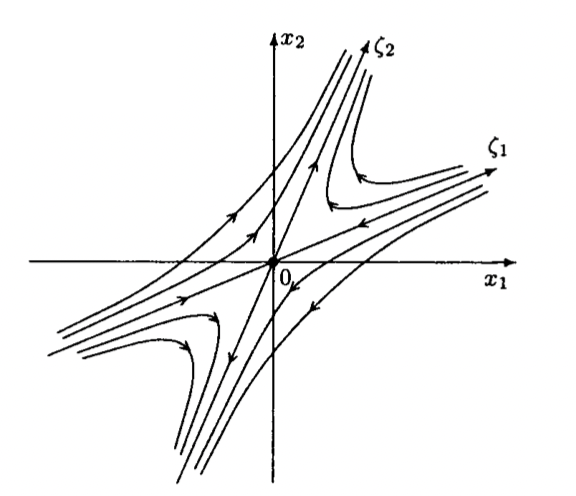
\includegraphics[scale=0.8]{sections/Sasha/images/autonom-casec.png}
            \caption{$\lambda_1 < 0 < \lambda_2$}
        \end{figure}
    
    \item Пусть \(\lambda_1 = \lambda_2 = \lambda\) и существует базис плоскости из собственных векторов $h_1, h_2$.
        Все действительные решения задаются формулой
        \[x(t) = e^{\lambda t} ( c_1 h_1 + c_2 h_2).\]
        \[\frac{dx_1}{dx_2}=\frac{c_1h_{11} + c_2h_{12}}{c_1h_{21} + c_2h_{22}} \text{ -- не зависит от } t\]
        Поэтому каждое такое решение описывает луч, выходящий из начала координат, причем движение по лучу при \(t \longrightarrow +\infty\) идет к нулю при \(\lambda < 0\) и от нуля при \(\lambda > 0\).\\
        При \(\lambda < 0\) положение равновесия $x = 0$ называется \textbf{устойчивым дикритическим узлом}, а при \(\lambda > 0\) \textbf{неустойчивым дикритическим узлом}. Схематически данный случай изображен на рисунке ниже.
        \begin{figure}[H]\label{autonom-cased}
            \centering
            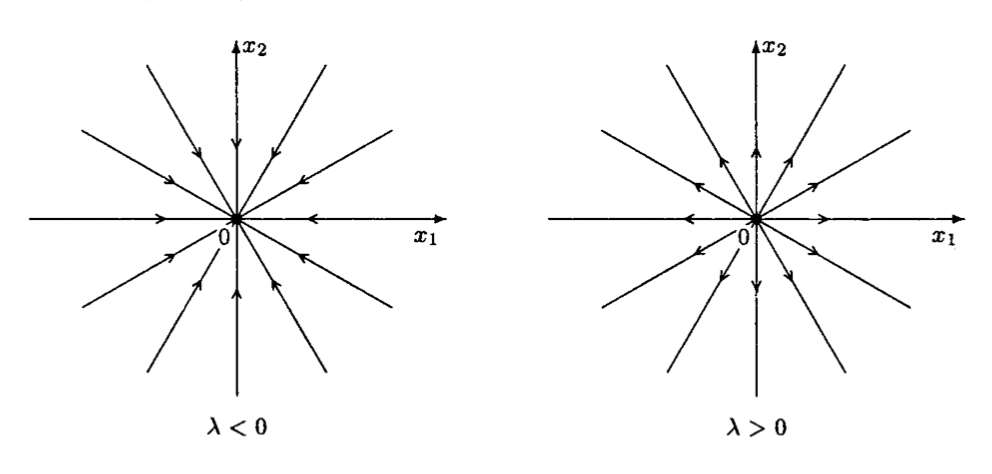
\includegraphics[scale=0.8]{sections/Sasha/images/autonom-cased.png}
            \caption{Дикритические узлы}
        \end{figure}

     \item Пусть \(\lambda_1 = \lambda_2 = \lambda\) и существует базис плоскости из собственного вектора $h_1$ и присоединенного к нему $h_{12}$.
        Все действительные решения задаются формулой
        \[x(t) = c_1 e^{\lambda t} h_1 + c_2 e^{\lambda t} (h_{12} + t h_1).\]
        В базисе из собственных векторов координаты решения \(x(t)\) системы~(\ref{autonom-sys-2d}) имеют вид
        \[\zeta_1 = (c_1 + c_2 t) e^{\lambda t}, \;\; \zeta_2 =  c_2 e^{\lambda t}.\]
        Для \(\lambda < 0\) получаем:
        \begin{itemize}
            \item при \(c_1 = c_2 = 0\) положение равновесия \(x = 0\);
            \item при \(c_1 \neq 0, c_2 = 0\) две полуоси \(\zeta_1 < 0, \zeta_1 > 0\) причем при \(t \longrightarrow +\infty\) идет к нулю; (т.е. получаем прямую $\zeta_1$).
            \item при \(c_2 \neq 0\) выносим t за скобки:
            \[x(t) = t\Big(c_2h_1e^{\lambda t} + \frac{1}{t}(c_1h_1e^{\lambda t} + c_2h_{2}e^{\lambda t})\Big) = \big(tc_2h_1+o(1)\big)e^{\lambda t} \text{ , где $o(1) \stackrel{t\to\infty}{\longrightarrow} 0$.}\]  Отсюда получаем, что $x(t)\; ||\; h_1$. При переходе в базис, в котором мы работали это значит $x(t)\; ||\; \zeta_1$. Множитель $t > 0$ при \(t \longrightarrow +\infty\) и $t < 0$ при \(t \longrightarrow -\infty\). Значит, траектория разворачивается в противоположном направлении. 
        \end{itemize}
        В случае \(\lambda < 0\) положение равновесия $x = 0$ называется \textbf{устойчивым вырожденным узлом} системы~(\ref{autonom-sys-2d}).
        
        В случае \(\lambda > 0\) траеткории получаются из описанных выше путем зеркального отображения относительно оси $\zeta_2$, а движение по ним при \(t \longrightarrow +\infty\) идет от начала координат.
        
        В случае \(\lambda > 0\) положение равновесия $x=0$ называется \textbf{неустойчивым вырожденным узлом}. Схематически фазовый портрет показан на рисунке ниже.
        \begin{figure}[H]\label{autonom-casee}
            \centering
            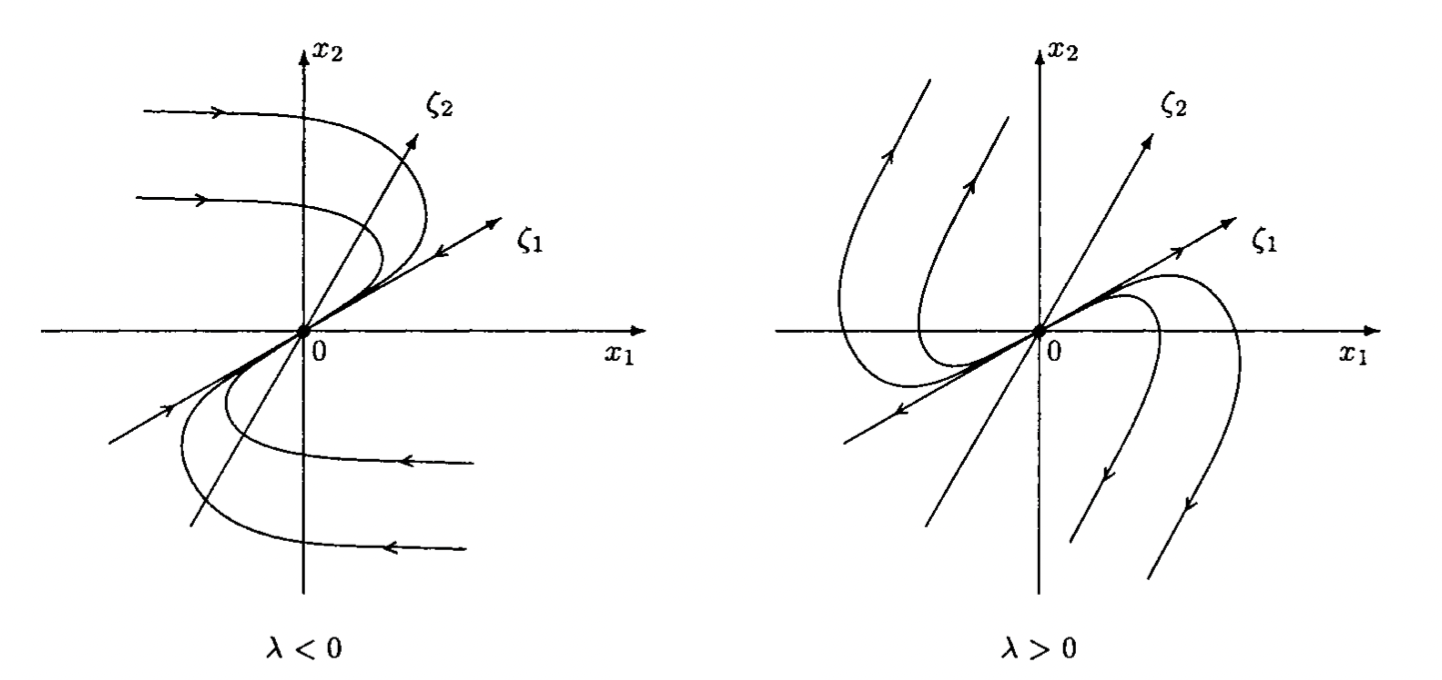
\includegraphics[scale=0.6]{sections/Sasha/images/autonom-casee.png}
            \caption{Вырожденные узлы}
        \end{figure}
    \end{enumerate}
    \item Случай комплексных $\lambda_1, \lambda_2$.\\
    Если \(\lambda_1 = \mu + i \nu\), где $\nu > 0$, то в силу действительности $A$ имеем \(\lambda_2 = \overline{\lambda_1} = \mu - i \nu\). Обозначим через \(h = h_1 - i h_2\) собственный вектор $A$ для $\lambda_1$, где $h_1, h_2$~--- действительные векторы. Тогда \(\overline{h} = h_1 + i h_2\) является собственным вектором для $\lambda_2$. Общее действительное решение~(\ref{autonom-sys-2d}) в этом случае имеет вид
    \[x(t) = c e^{\lambda_1 t}h + \overline{c} e^{\overline{\lambda_1}t} \overline{h},\]
    где $c$~--- произвольная комплексная константа.
    
    Если положить 
    \[c = |c|e^{i\varphi}, \varphi \in [0; 2\pi),\]
    то \(\overline{c} = |c| e^{-i\varphi}\) и общее решение преобразуется к виду \[x(t) = 2 |c|e^{\mu t}[\cos{(\varphi + \nu t)} h_1 + \sin{(\varphi + \nu t)} h_2].\]
    Так как $h_1$ и $h_2$~--- линейно независимы, то взяв их в качестве нового базиса плоскости координаты решения в этом базисе будут иметь вид
    \[\zeta_1(t) = 2 |c|e^{\mu t} cos(\varphi + \nu t), \;\; \zeta_2(t) = 2 |c|e^{\mu t}sin(\varphi + \nu t).\]
    Положив \(r(t) = 2 |c| e^{\nu t}, \psi(t) = \varphi + \nu t\), отсюда получаем уравнение траекторий в полярных координатах $r, \psi$
    \[r(t) = 2|c| \cdot \exp\Big(\mu \frac{\psi - \varphi}{\nu}\Big).\]
    
    При $c \neq 0, \mu \neq 0$ фазовые траектории представляют собой кривые типа логарифмических спиралей, а при $\mu = 0$~--- кривые типа эллипсов.
    \begin{enumerate}
    \item Пусть $\mu < 0$.\\
        Тогда при $c = 0$ получаем положение равновесия $x=0$, а при $c \neq 0$ фазовая точка по спирали \underline{движется} к $x=0$ при \(t \longrightarrow +\infty\) , так как $r(t) \longrightarrow +0, \psi(t) \longrightarrow +\infty$ при \(t \longrightarrow +\infty\).
        
        Направление закручивания определяется направлением фазовой скорости. Например, можно рассмотреть точку $(0, 1)$ и тогда $f(x)$ будет иметь компоненты $a_{12}, a_{22}$. Возможные два различных фазовых портрета в этом случае схематически показаны на рисунке ниже
        \begin{figure}[H]\label{autonom-compla}
                \centering
                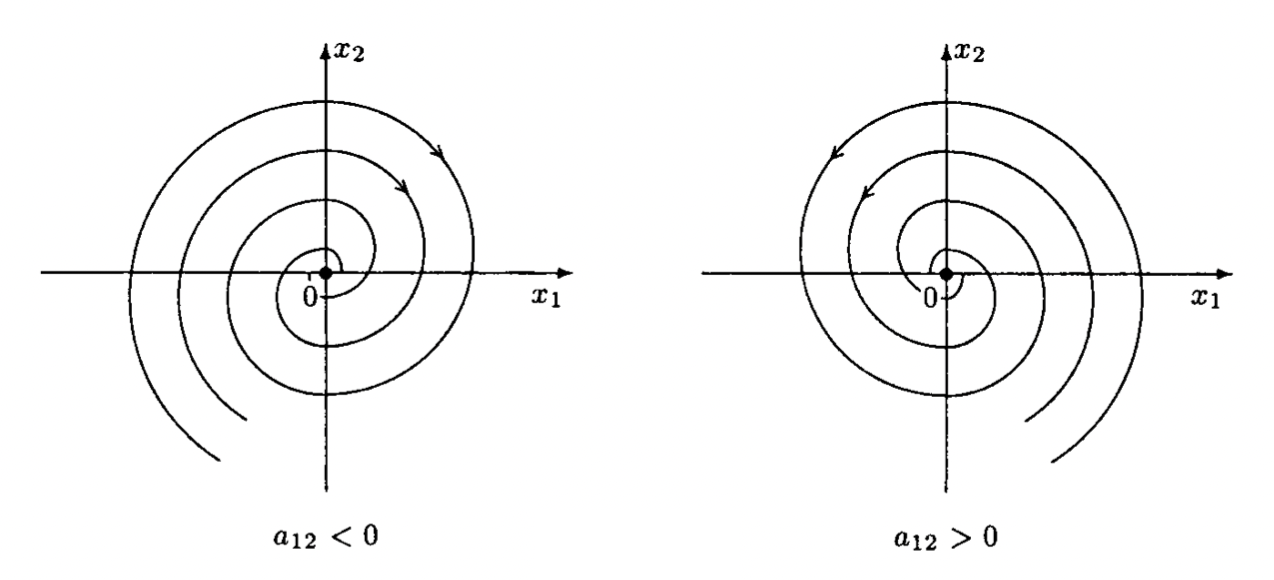
\includegraphics[scale=0.6]{sections/Sasha/images/autonom-compla.png}
                \caption{}
        \end{figure}
        Положение равновесия $x=0$ в этом случае называется \textbf{устойчиывым фокусом} системы.
    
    \item Пусть $\mu > 0$.\\
        Тогда при $c = 0$ получаем положение равновесия $x=0$, а при $c \neq 0$ фазовая точка по спирали \underline{удаляется от} $x=0$ при \(t \longrightarrow +\infty\), так как $r(t) \longrightarrow +\infty, \psi(t) \longrightarrow +\infty$ при \(t \longrightarrow +\infty\).
        
        В этом случае положение равновесия $x=0$ называется \textbf{неустойчивым фокусом} системы. Возможные в этом случае два различных фазовых портрета схематически показаны на рисунке ниже.
        \begin{figure}[H]\label{autonom-complb}
                \centering
                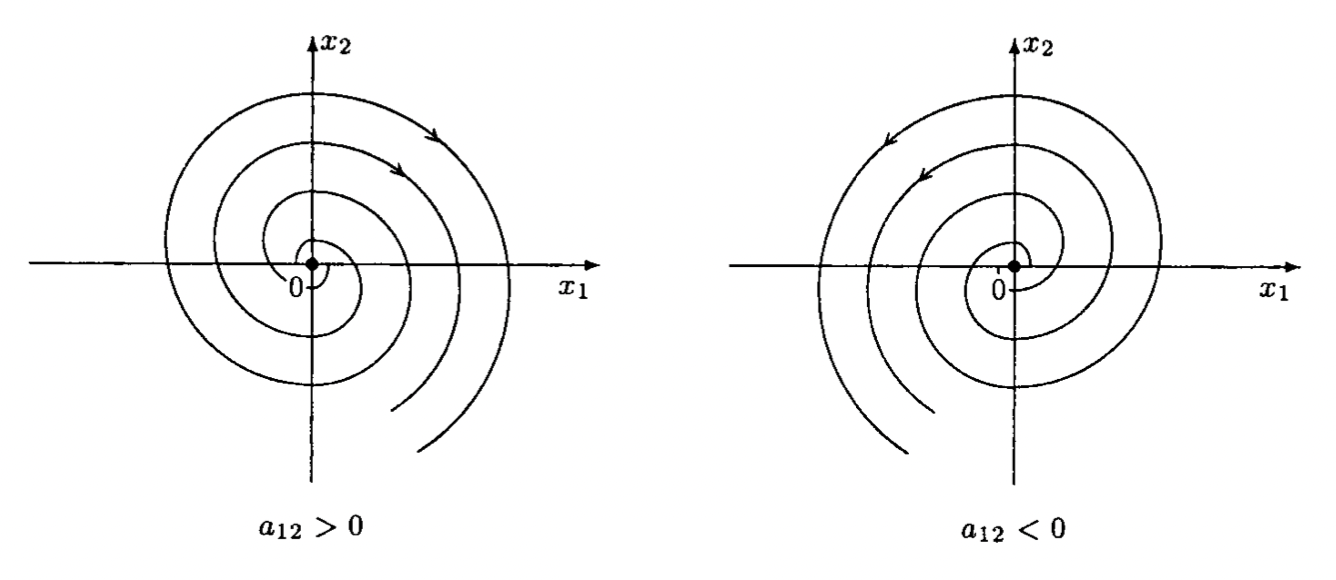
\includegraphics[scale=0.6]{sections/Sasha/images/autonom-complb.png}
                \caption{}
        \end{figure}
    \item Пусть $\mu = 0$.\\
        Тогда в произвольном базисе $h_1$ и $h_2$ при $c \neq 0$ траектории — кривые типа эллипса, а при $c = 0$~--- положение равновесия $x=0$. В этом случае положение равновесия называется \textbf{центром для системы}~(\ref{autonom-sys-2d}). В зависимости от направления обхода эллипсов возможные фазовые портреты схематиески изображены на рисунке ниже.
        \begin{figure}[H]\label{autonom-complc}
            \centering
            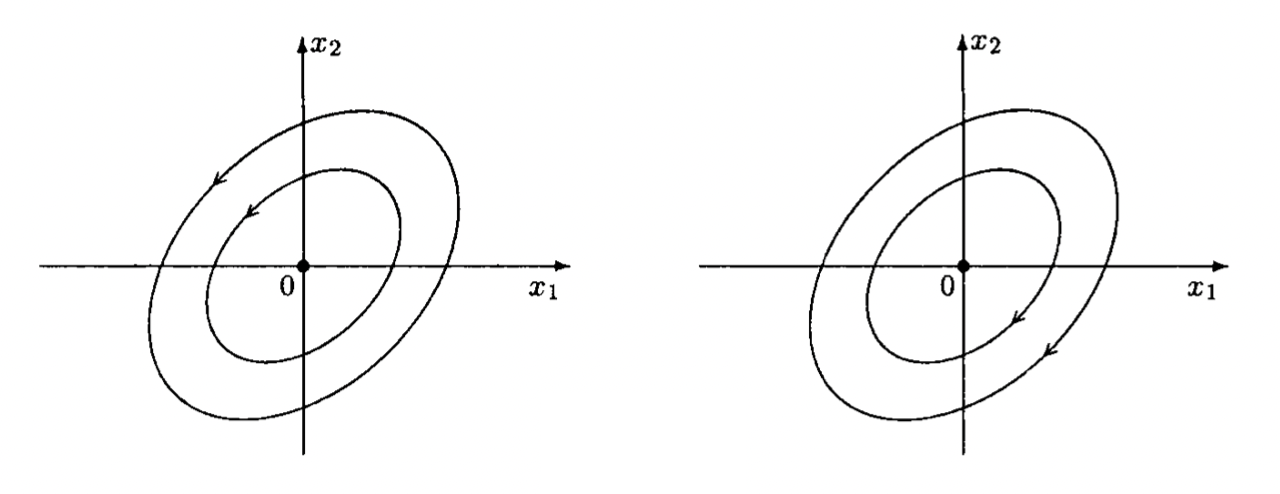
\includegraphics[scale=0.6]{sections/Sasha/images/autonom-complc.png}
            \caption{}
        \end{figure}
    \end{enumerate}
\end{enumerate}

Таким образом, для простой линейной автономной системы существует всего (хах, "всего") тринадцать различных фазовых портретов.

\paragraph{Случай сложной системы}
Напомню, что система~(\ref{autonom-sys-2d}) называется сложной если матрица $A$ вырождена.

\begin{enumerate}[label=(\alph*)]
    \item Пусть $\lambda_1 \neq 0, \lambda_2 = 0$.\\
        Тогда \(\zeta_1(t) = c_1 e^{\lambda_1 t}, \;\zeta_2(t) = c_2\). Отсюда ясно, что все точки прямой $\zeta_1= 0$ являются положениями равновесия и что оба луча луча каждой прямой $\zeta_2(t) = c_2$ являются траекториями~(\ref{autonom-sys-2d}).
        
        В зависимости от знака $\lambda_1$ движенеи по ним при \(t \longrightarrow +\infty\) идет либо к прямой $\zeta_1= 0$ либо от нее. В зависимости от знака $\lambda_1$ возможны два схематически представленных на рисунке ниже
        \begin{figure}[H]\label{autonom-triviala}
            \centering
            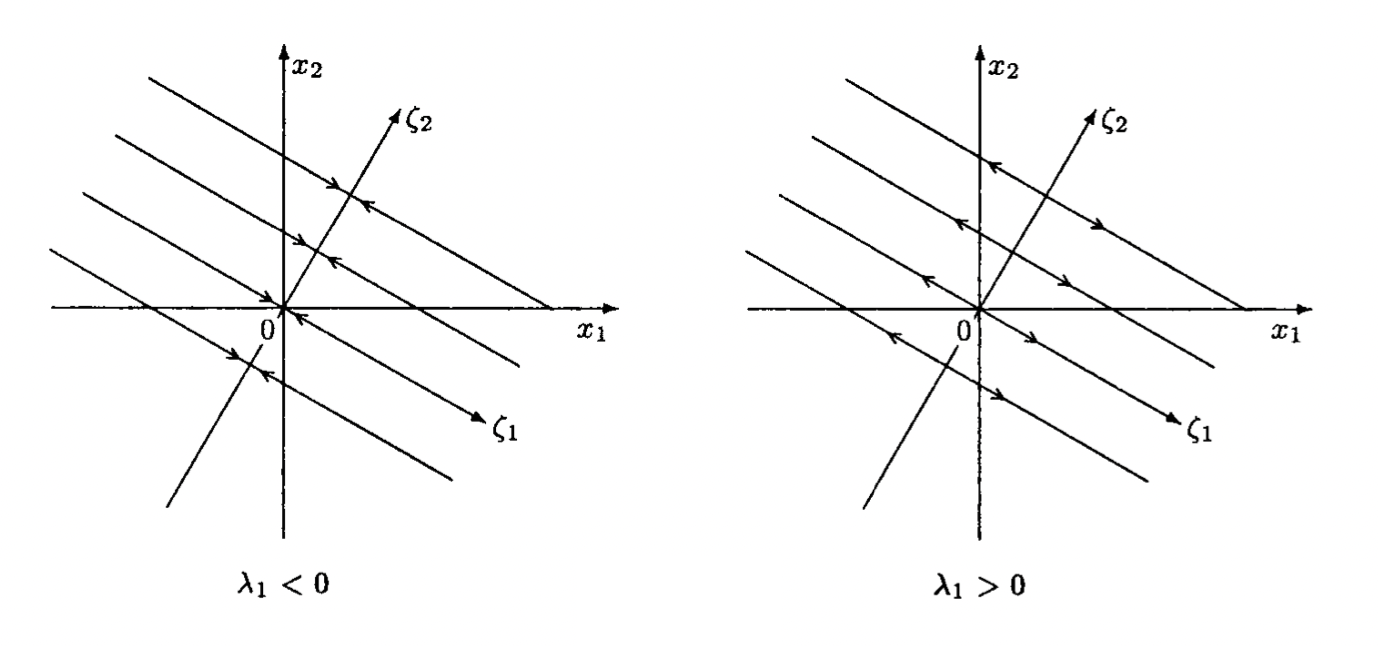
\includegraphics[scale=0.6]{sections/Sasha/images/autonom-triviala.png}
            \caption{}
        \end{figure}
        
    \item Пусть $\lambda_1 = \lambda_2 = 0$.\\
        Если матрица $A$ нулевая,  то каждая точка плоскости является положением равновесия. 
        
        Если же $A$ ненулевая, то существует базис плоскости из собственного вектора $h_1$ и присоединенного к нему $h_2$. В этом базисе  решение имеет координаты 
        \[\zeta_1(t) = c_1 + c_2 t, \;\; \zeta_2(t) = c_2.\]
        Отсюда ясно, что все точки прямой $\zeta_2= 0$ являются положениями равновесия. Каждая из прямых $\zeta_2 = c$ является траекторией и при \(t \longrightarrow +\infty\) движение по ним идет слева направо при $\zeta_2>0$ и справа налево при $\zeta_2<0$. Изображено на рисунке ниже.
        \begin{figure}[H]\label{autonom-trivialb}
            \centering
            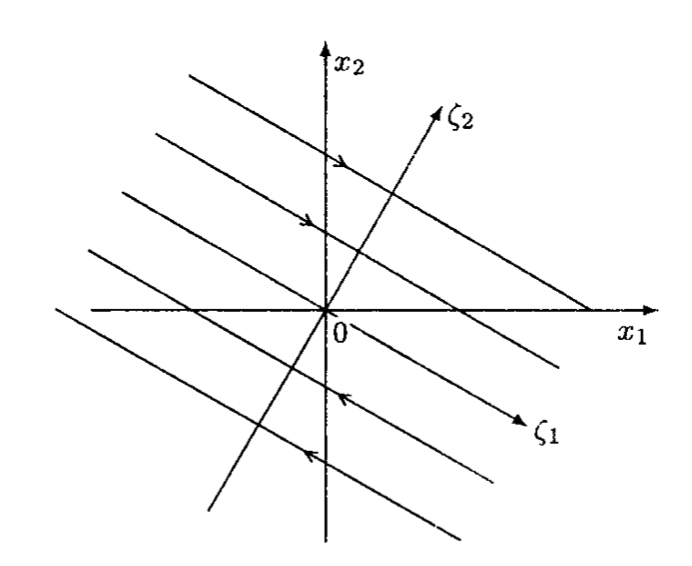
\includegraphics[scale=0.6]{sections/Sasha/images/autonom-trivialb.png}
            \caption{}
        \end{figure}
\end{enumerate}

Таким образом, для сложной линейной автономной системы существует всего четыре различных фазовых портрета.
